\documentclass[preprint]{sigplanconf}

% The following \documentclass options may be useful:
%
% 10pt          To set in 10-point type instead of 9-point.
% 11pt          To set in 11-point type instead of 9-point.
% authoryear    To obtain author/year citation style instead of numeric.

\usepackage{amsmath}
\usepackage{graphicx}

\begin{document}

\conferenceinfo{ICFP '13}{date, Boston} 
\copyrightyear{2013} 
\copyrightdata{[to be supplied]} 

\titlebanner{Red-Black Tree Deletion}        % These are ignored unless
\preprintfooter{Presents the missing method of Okasaki's red-black trees.}   % 'preprint' option specified.

\title{Deletion: The Curse of the Functional Red-Black Tree}
\subtitle{Functional Pearl}

\authorinfo{Kimball Germane\and Matt Might}
           {University of Utah}
           %{Email2/3}

\maketitle

\begin{abstract}
Red-black trees were properly introduced into the functional world when Okasaki gave a succinct method of element insertion. Even still, deletion has remained complex, requiring the consideration of a litany of rebalancing cases and contingencies. With such conceptual impenetrability, it's no wonder that authors have turned to advanced type systems and formal methods to ensure correctness. This has relegated workaday functional programmers to be mere implementation consumers. We aim to democratize deletion by providing a method that is intuitive, succinct, and obviously correct.
\end{abstract}

\category{CR-number}{subcategory}{third-level}

\terms
red-black tree, delete, data structure

\keywords
red-black tree, delete, data structure

\section{Introduction}

When looking for a data structure to back a functional implementation of sets, red-black trees--a type of balanced binary search tree--are a natural choice. Common set operations, such as membership testing and persistent addition, map naturally to their native operations of search and insertion. And, speaking of maps, minor modifications can turn a set membership test into a map lookup operation and set addition into map extension.

The usefulness of red-black trees stems from their balanced nature. A red-black tree is a binary tree in which each node is colored red or black, and which satisfies the local property that
\begin{enumerate}
\item every red node has two black children,
\end{enumerate}
and the global property that
\begin{enumerate}
\setcounter{enumi}{1}
\item every path from the root to a leaf\footnote{For our purposes, leaf nodes do not contain data and are colored black.} node contains the same number of black nodes.
\end{enumerate}
These conditions guarantee that the longest path from root to leaf can be no more than twice the shortest (the only difference being individual red nodes interspersed along the way), and so the worst-case penalty of locating an element as part of a red-black tree operation is a reasonable constant factor over that of a perfectly balanced tree.

Red-black trees were properly introduced into the functional world when Okasaki gave a succinct method of element insertion \cite{okasaki1999functional}. Even still, deletion has remained complex, requiring the consideration of a litany of cases and contingencies. Because of the lack of an overarching intuition, ensuring correctness has become a burden. To cope with this, authors have turned to advanced type systems \cite{kahrs2001red} and formal methods \cite{appel2011efficient}. The apparent difficulty of bearing the onus of correctness has relegated workaday functional programmers to be mere implementation consumers or to go without if their functional language lacks one.

This situation should seem familiar. Before Okasaki's functional treatment, insertion into red-black trees suffered the same impenetrability. However, clarification did not come from a reference implementation. In addition to providing a functional treatment, Okasaki succeeded in adding intuition to something considered to be intricate and error-prone. The net effect of his contribution is not code so short that it is easily memorizable but a concept so elegant and natural that, from it, the code is easily derivable--very befitting of its pearl namesake.

We aim to democratize deletion in a similar way by providing a method that is intuitive, succinct, and obviously correct.

As an example to introduce rigorous yet informal methods to reason about correctness, we briefly review Okasaki's functional insertion.

\section{Insertion}

Okasaki accomplished insertion by means of the recursive \texttt{insert} function and the \texttt{balance} helper function.

Using a bit of syntactic sugar on top of Racket \cite{plt-tr1}, we can express the \texttt{insert}\footnote{We use the variable \texttt{k} to denote the value to insert to avoid later confusion.} function with
\begin{verbatim}
(define (insert t k)
  (match t
    [(L) (R (L) k (L))]
    [(N c a x b)
     (switch-compare
       (k x)
       [< (balance (N c (insert a k) x b))]
       [= (N c a x b)]
       [> (balance (N c a x (insert b k)))])]))
\end{verbatim}
where \texttt{balance} yet remains undefined.

This definition of \texttt{insert} unilaterally colors each newly-added node red, but this may create a problem: if the parent of this new node is red, this action violates the local property. Okasaki persists in the face of this possibility, reasoning that it is easier to resolve a violation of the local property than the global one. This is achieved by the \texttt{balance} function which takes trees of one of the forms of
\begin{center}
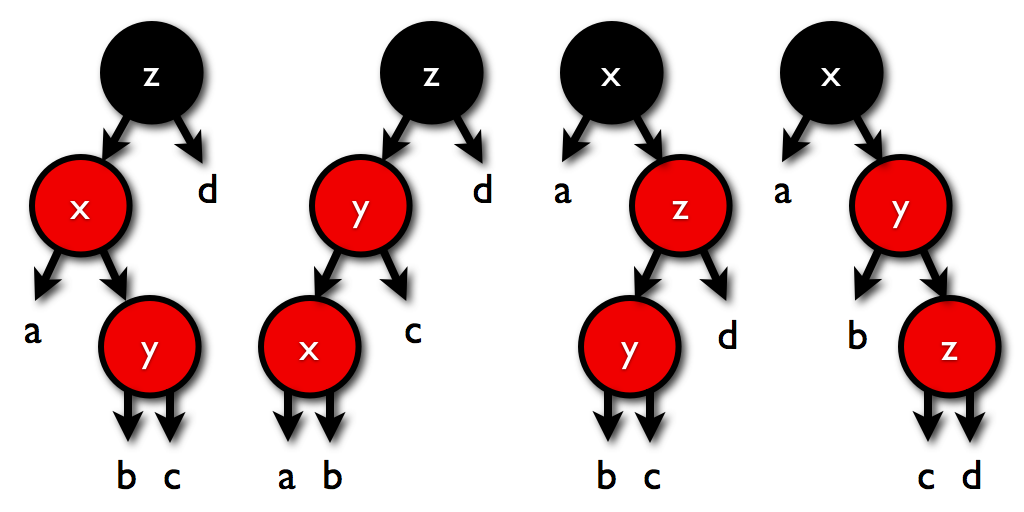
\includegraphics{four-cases.pdf}
\end{center}
and transforms them into
\begin{center}
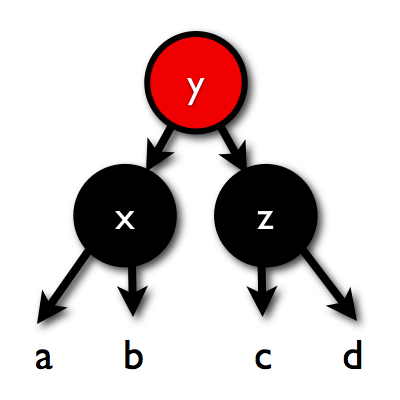
\includegraphics{four-cases-resolved.pdf}
\end{center}
Expressed in code, this is equally concise:
\begin{verbatim}
(define-match balance
  [(or (B (R (R a x b) y c) z d)
       (B (R a x (R b y c)) z d)
       (B a x (R (R b y c) z d))
       (B a x (R b y (R c z d))))
   (R (B a x b) y (B c z d))])
\end{verbatim}

In order to verify that we are not beguiled by the elegance of this transformation, we need to ensure that it has three properties, that as it resolves one violation: it preserves correct tree ordering; it does not unduly introduce other local property (red-red) violations; and it does not introduce any global property (height) violations.

It is routine to verify that this transformation preserves a correct tree ordering, but no less important for it. We will say little about order preservation, but it is critical to verify for each transformation we introduce.

Next, we verify that this transformation doesn't introduce any red-red violations unduly. It clearly resolves the red-red violation of its design, but we must consider any introductions of the same. We observe that, below this section of the tree, the subtrees $a$, $b$, $c$, ande $d$ are compatible with their newly-assigned parents, no matter the colorings of their roots. However, consider the parent of this section of the tree. If the parent is red, then this transformation \emph{introduces} exactly the same kind of red-red violation it resolved, only further up the tree. It is here that we rely on the recursive nature of \texttt{insert} and the application of \texttt{balance} at each step. We reason inductively that each violation introduced in this way will be handled by the same mechanism.

Finally, we verify that the transformation does not introduce any height violations. We do this by ensuring that the number of black nodes this section of the tree contributes to each path through it is the same before and after it occurs. Like the first property, verifying this is routine but nevertheless critical.

The final stop of Okasaki's insertion algorithm is to blacken the root of the tree, which is benign in all cases. This requires a small modification of \texttt{insert} to 
\begin{verbatim}
(define (insert t k)
  (define (ins t k)
    (match t
      [(L) (R (L) k (L))]
      [(N c a x b)
       (switch-compare
         (k x)
         [< (balance (N c (insert a k) x b))]
         [= (N c a x b)]
         [> (balance (N c a x (insert b k)))])]))
  (blacken (ins t k)))
\end{verbatim}
with \texttt{blacken} given by
\begin{verbatim}
(define-match blacken
  [(N _ a x b) (N 'B a x b)])
\end{verbatim}

Our formulation of the red-black invariants allows trees to have red roots in some cases, so our root-coloring policy is more conservative, only blackening if the red-black construction demands it. This leads only to a change to \texttt{blacken}, which is now
\begin{verbatim}
(define-match blacken
  [(or (R (R? a) x b)
       (R a x (R? b)))
   (B a x b)]
  [t t])
\end{verbatim}

\section{Deletion}

Insertion into binary trees has the advantage that new nodes are added only to the fringe, whereas deletion might also target interior nodes. With deletion, we only have to be slightly clever to reduce the latter situation to the former: when deleting a value that resides in an interior node, replace that node's value with the minimum value of its right subtree, and delete that value from that subtree.\footnote{An alternative is to distinguish left subtrees and use the maximum element. By considering right subtrees, we get a \texttt{min-element} function for free, which is useful for priority queues.} This strategy contains a reference to deletion itself, so, like insertion, this approach can be defined recursively. Roughly, we express it by
\begin{verbatim}
(define (delete t k)
  (match t
    [(N c a x b)
     (switch-compare
       (k x)
       [< (N c (delete a k) x b)]
       [= (let ([v (min-element b)])
            (N c a v (delete b k)))]
       [> (N c a x (delete b k))])]))
\end{verbatim}
Essentially, this algorithm first locates the given value with a simple binary search and then applies our strategy, invoking itself. By enhancing this approach to account for red-black properties, we obtain a sound, persistent method of deletion from red-black trees!

We start by considering the genuine base cases of the delete algorithm: the configurations that don't entail a node with a right subtree from which we can extract the minimum element.

\begin{itemize}

\item If the value to delete is not present in the tree, the search will terminate on an empty tree. This presents no difficulty: the empty tree remains unchanged after the removal of any element.
\begin{center}
\includegraphics{empty-step.pdf}
\end{center}
As a case for the \texttt{delete} function, this can be written
\begin{verbatim}
[(L) (L)]
\end{verbatim}

\item Because red nodes do not contribute to the height of the tree, we can soundly remove them from the bottom. Therefore, a single red node becomes the empty tree.
\begin{center}
\includegraphics{single-red-step.pdf}
\end{center}
As a case for the \texttt{delete} function, this is
\begin{verbatim}
[(R (L) (== k) (L)) (L)]
\end{verbatim}

\item A red node with a black-rooted left subtree
\begin{center}
\includegraphics{red-black-left-subtree.pdf}
\end{center}
violates the global property and cannot occur.

\item A black node with a red-rooted left subtree becomes the subtree itself, only black-rooted.
\begin{center}
\includegraphics{black-red-left-subtree-step.pdf}
\end{center}
Conceptually, we are only removing a single red node from the tree. Absent subtree merging, this is completely straightforward. As a case for the \texttt{delete} function, this is
\begin{verbatim}
[(B (R a x b) (== k) (L)) (B a x b)]
\end{verbatim}

\item Finally, a black node with no left or right subtree
\begin{center}
\includegraphics{single-black.pdf}
\end{center}
presents us with a challenge. The paths that end at one of its leaves accumulate two black nodes from this portion of the tree--one from the node itself and one from the leaf. Thus, the careless excision of it would violate the global property by altering the height of the tree. Repurposing some wisdom from Okasaki, perhaps we should attempt to preserve the global property at the expense of something more local. We do this by introducing the double-black color (\texttt{BB}) of which both branches
\begin{center}
\includegraphics{double-black-tree.pdf}
\end{center}
and leaves
\begin{center}
\includegraphics{double-black-leaf.pdf}
\end{center}
can be classified. For accounting purposes, a double-black node contributes two black nodes to any path that travels through it. With this intuition, it is obvious what a lone black node becomes after deletion:
\begin{center}
\includegraphics{single-black-step.pdf}
\end{center}

\end{itemize}

Of course, once this substitution is made, we no longer have a red-black tree, and must reconcile our newly-created tree with the red-black properties. Having adopted Okasaki's initial approach, it seems only natural to apply the rest of it, if possible.

Recall that \texttt{insert} adds a red node to the tree, possibly introducing a red-red violation, and that \texttt{balance} resolves a red-red violation locally, possibly introducing another higher in the tree. Because \texttt{insert} is recursive, it can apply \texttt{balance} at each level, pushing red-red violations to the root where they can be resolved unequivocally.

We now find wisdom in formulating \texttt{delete} recursively, as we can use the same strategy. Instead of introducing red-red violations to be resolved by \texttt{balance}, we introduce double-black nodes to be discharged by \texttt{rotate}.

Our \texttt{delete} function is now defined as
\begin{verbatim}
(define (delete t k)
  (match t
    [(L) (L)]
    [(R (L) (== v) (L)) (L)]
    [(B (L) (== v) (L)) (BB)]
    [(B (R a x b) (== v) (L)) (B a x b)]
    [(N c a x b)
     (switch-compare
       (k x)
       [< (rotate (N c (delete a k) x b))]
       [= (let ([v (min-element b)])
            (rotate (N c a v (delete b k))))]
       [> (rotate (N c a x (delete b k)))])]))
\end{verbatim}
with \texttt{rotate} still undefined.

The \texttt{rotate} function rearranges trees whose root node has a double-black child and either discharges the double-black node immediately or moves it to the root of the tree. Surprisingly, it need only be applied to three distinct cases and their reflections.

The first case is a red-rooted tree with a double-black child. This condition is sufficient to conclude that the other child is black--not red--and is a node--not a leaf. In this case, the double black node can be discharged immediately with the rotation
\begin{center}
\includegraphics{BB-R-B.pdf}
\end{center}
We can verify that the number of black nodes this tree contributes to each path through it is unchanged by this rotation, so it doesn't disrupt the global property. However, it possibly introduces a red-red violation. Fortunately, this is no matter: we can \texttt{balance} it away! As a case for the \texttt{rotate} function, we can express the rotation of this case and its reflection by
\begin{verbatim}
[(R (BB? a) x (B b y c))
 (balance (B (R (-B a) x b) y c))]
[(R (B a x b) y (BB? c))
 (balance (B a x (R b y (-B c))))]
\end{verbatim}
where \texttt{BB?} matches a double-black node or leaf without deconstructing it and \texttt{-B} demotes a double-black node or leaf to its black counterpart (and is undefined on red nodes).

The second case is a black-rooted tree with a double-black child and a black child, necessarily a node. The situation is identical to the previous case but for the additional black node contributed by the root to each path. This additional black node prevents us from discharging the double-black node immediately so we defer its resolution by arranging it at the root.
\begin{center}
\includegraphics{BB-B-B.pdf}
\end{center}
As cases for the \texttt{rotate} function, this is
\begin{verbatim}
[(B (BB? a) x (B b y c))
 (balance (BB (R (-B a) x b) y c))]
[(B (B a x b) y (BB? c))
 (balance (BB a x (R b y (-B c))))]
\end{verbatim}
This rotation presents a minor complication: because of its double-black root, the red-red violation can no longer be handled by \texttt{balance}. We cope with this by extending \texttt{balance} over just these situations. This is as simple as adding cases for trees of the form
\begin{center}
\includegraphics{two-cases-extended.pdf}
\end{center}
and transforming each of them to
\begin{center}
\includegraphics{two-cases-extended-resolved.pdf}
\end{center}
Unlike the original cases of \texttt{balance}, there is no way that this transformation can introduce a red-red violation; it doesn't introduce any red nodes! In fact, the need to balance is almost preferable here since the operation itself would discharge the double-black node!

The third and final case is a black-rooted tree with a double-black child and a red child, necessarily a node.
\begin{center}
\includegraphics{BB-B-R.pdf}
\end{center}
It is hopeless to attempt to rearrange this tree to satisfy, simultaneously, ordering, red-red violations modulo \texttt{balance}, and height adjustments modulo \texttt{rotate}. Notice, however, that there is only one possibility for the children of the red node: they are both black and both necessarily nodes. Considering these also gives us just enough to satisfy all the constraints:
\begin{center}
\includegraphics{BB-B-R-B-B.pdf}
\end{center}
Once again, the introduction of a red-red violation is a possibility, only this time, it is deeper in the tree. We balance where it could occur, noting that a balance could not introduce another red-red violation here, so we need not handle the possibility. As cases for the \texttt{rotate} function, this is expressed by
\begin{verbatim}
[(B (BB? a) x (R (B b y c) z (B? d)))
 (B (balance (B (R (-B a) x b) y c)) z d)]
[(B (R (B? a) x (B b y c)) z (BB? d))
 (B a x (balance (B b y (R c z (-B d)))))]
\end{verbatim}

We might ask whether a double black node will reach the top before resolution. Such an occurrence would not be fatal since we could soundly demote it to a black node at the root. This would require exposing the \texttt{blacken} function to the transient double-black color, but in the interest of double-black containment, we opt for a different approach. Recall that the final step of \texttt{insert} is to to blacken the root if necessary. We apply the dual of this step so that the first step of \texttt{delete} is to redden the root if possible. If it can be reddened, then the full tree will fall under the first case and a double-black node can be discharged at the top. If it cannot be reddened, then at least one of its children is red. If the value to be deleted is found in the red-rooted subtree, the first case of rotation applies to the subtree. If not, the third case of rotation applies to the entire tree. Thus, in no case can a double-black node reach the root. [Make this structured and not a block of text?]

With proper syntax in hand, the essence of this algorithm is incredibly succinct.

\begin{verbatim}
(define-match blacken
  [(or (R (R? a) x b)
       (R a x (R? b)))
   (B a x b)]
  [t t])

(define-match redden
  [(B (B? a) x (B? b))
   (R a x b)]
  [t t])

(define-match min
  [(L) (error 'min "empty tree")]
  [(N _ (L) x _) x]
  [(N _ a _ _) (min a)])

(define-match balance
  [(or (B (R (R a x b) y c) z d)
       (B (R a x (R b y c)) z d)
       (B a x (R (R b y c) z d))
       (B a x (R b y (R c z d))))
   (R (B a x b) y (B c z d))]
  [(or (BB (R a x (R b y c)) z d)
       (BB a x (R (R b y c) z d)))
   (B (B a x b) y (B c z d))]
  [t t])

(define-match -B
  [(BB) (L)]
  [(BB a x b) (B a x b)]
  [a (error '-B "unsupported node ~a" a)])

(define-match rotate
  [(R (BB? a) x (B b y c))
   (balance (B (R (-B a) x b) y c))]
  [(R (B a x b) y (BB? c))
   (balance (B a x (R b y (-B c))))]
    
  [(B (BB? a) x (B b y c))
   (balance (BB (R (-B a) x b) y c))]
  [(B (B a x b) y (BB? c))
   (balance (BB a x (R b y (-B c))))]
    
  [(B (BB? a) x (R (B b y c) z (B? d)))
   (B (balance (B (R (-B a) x b) y c)) z d)]
  [(B (R (B? a) x (B b y c)) z (BB? d))
   (B a x (balance (B b y (R c z (-B d)))))]
    
  [t t])

(define (delete t v cmp)
  (define (del t v cmp)
    (match t
      [(L) (L)]
      [(R (L) (== v) (L))
       (L)]
      [(B (L) (== v) (L))
       (BB)]
      [(B (R a x b) (== v) (L))
       (B a x b)]
      [(N c a x b)
       (switch-compare
        (cmp v x)
        [< (rotate (N c (del a v cmp) x b))]
        [= (let ([v (min b)])
             (rotate (N c a v (del b v cmp))))]
        [> (rotate (N c a x (del b v cmp)))])]))
  (del (redden t) v cmp))
\end{verbatim}

\section{More}

We have, seemingly for the sake of simplicity, omitted the black-rooted tree with a red-rooted right subtree as a base case of the \texttt{delete} function, instead letting this case be handled by the recursive step. When dealing with unrestricted binary trees, this omission alters the time complexity of the algorithm. For, consider the number of invocations of \texttt{delete} on
\begin{center}
\includegraphics{right-cascade.pdf}
\end{center}
with and without this base case. Fortunately, the restrictions of red-black trees impose a tight bound on the maximum recursion depth of \texttt{delete}. Specifically, the global property ensures that
\begin{center}
\includegraphics{black-red-right-subtree-unbounded.pdf}
\end{center}
is at worst
\begin{center}
\includegraphics{black-red-right-subtree-bounded.pdf}
\end{center}
and that
\begin{center}
\includegraphics{red-black-right-subtree.pdf}
\end{center}
cannot occur. This limits the the opportunities for recursion to appear at most twice. The first appears when the candidate value resides in an interior node, and the deletion recurs on the right subtree. The second appears when the minimum element in that subtree resides in a node with a right subtree, and the deletion recurs on that subtree. The global property ensures that this subtree is a singleton, so the recursion is cut off at this point.

\section{Conclusion}



%\appendix
%\section{Appendix Title}

%This is the text of the appendix, if you need one.

%\acks

%Acknowledgments, if needed.

% We recommend abbrvnat bibliography style.

\bibliographystyle{abbrvnat}
\bibliography{red-black-pearl}

% The bibliography should be embedded for final submission.

%\begin{thebibliography}{}
%\softraggedright

%\bibitem[Smith et~al.(2009)Smith, Jones]{smith02}
%P. Q. Smith, and X. Y. Jones. ...reference text...

%\end{thebibliography}

\end{document}







